\documentclass[tikz,border=2pt,11pt]{standalone}
\usepackage{amsmath}
\usepackage{amssymb}
\usepackage{mathrsfs}
\usepackage{graphicx}
\usepackage{xcolor}
\newcommand{\Fp}{\mathbb F_p}
\newcommand{\Zp}{\mathbb Z_p}
\newcommand{\Qp}{\mathbb Q_p}
\newcommand{\Z}{\mathbb Z}
\newcommand{\Q}{\mathbb Q}
\newcommand{\F}{\mathbb F}
\newcommand{\cO}{\mathcal O}
\newcommand{\cG}{\mathcal G}
\newcommand{\cD}{\mathcal D}
\newcommand{\cM}{\mathcal M}
\DeclareMathOperator{\GL}{GL}
\DeclareMathOperator{\Gal}{Gal}
\DeclareMathOperator{\Ext}{Ext}
\DeclareMathOperator{\Hom}{Hom}
\DeclareMathOperator{\Lie}{Lie}
\DeclareMathOperator{\Aut}{Aut}
\DeclareMathOperator{\Spec}{Spec}
\DeclareMathOperator{\Spf}{Spf}
\DeclareMathOperator{\Spa}{Spa}
\DeclareMathOperator{\Spd}{Spd}
\DeclareMathOperator*{\colim}{colim}
\DeclareMathOperator{\coker}{coker}
\DeclareMathOperator{\cofib}{cofib}
\DeclareMathOperator{\fib}{fib}
\DeclareMathOperator{\RHom}{RHom}
\newcommand{\RGamma}{R\Gamma}
\newcommand{\LK}[1]{L_{K(#1)}}
\newcommand{\LN}[1]{L_{#1}}
\begin{document}
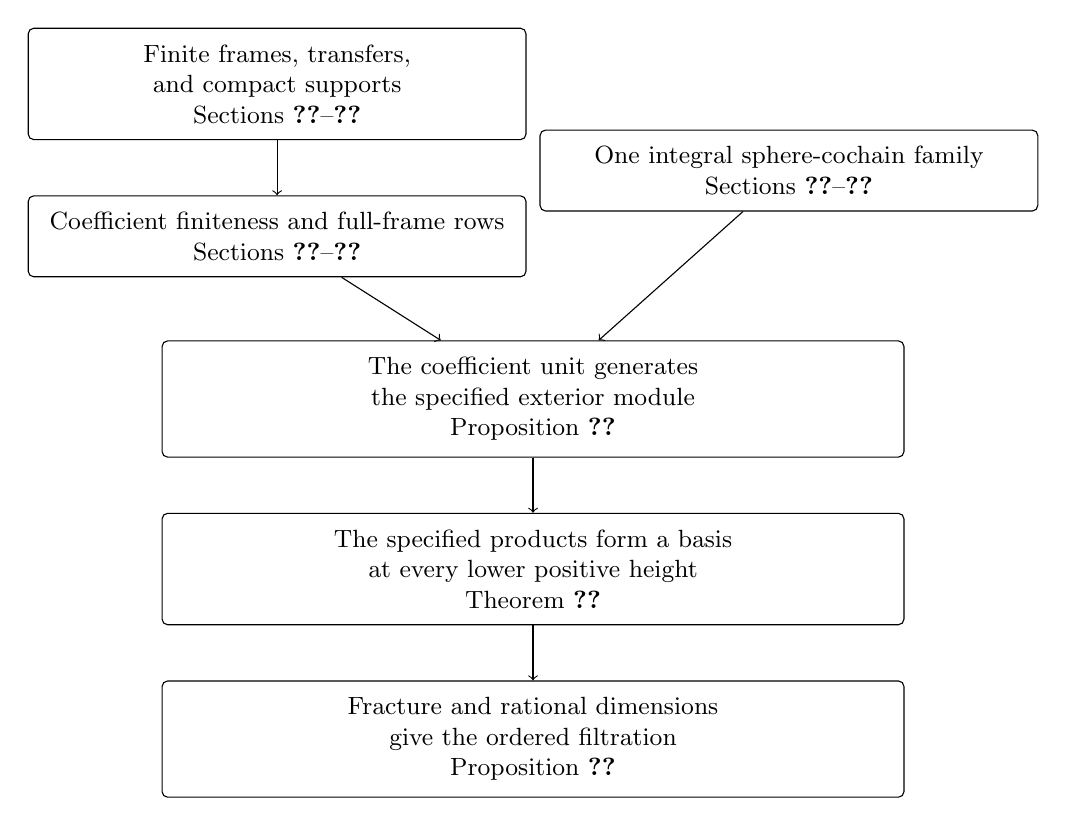
\begin{tikzpicture}[
  every node/.style={align=center,font=\small},
  box/.style={draw,rounded corners=2pt,inner sep=6pt,text width=5.9cm}
]
\node[box] (geometry) at (-3.25,0)
  {Finite frames, transfers, and compact supports\\
   Sections~\ref{sec:rings}--\ref{sec:support}};
\node[box,anchor=north] (finiteness)
  at ([yshift=-7mm]geometry.south)
  {Coefficient finiteness and full-frame rows\\
   Sections~\ref{sec:compact}--\ref{full:section}};
\node[box] (classes) at (3.25,-1.1)
  {One integral sphere-cochain family\\
   Sections~\ref{sec:constants}--\ref{sec:generators}};
\node[box,text width=9cm,anchor=north] (module)
  at ([xshift=3.25cm,yshift=-8mm]finiteness.south)
  {The coefficient unit generates\\the specified exterior module\\
   Proposition~\ref{prop:constant-module}};
\node[box,text width=9cm,anchor=north] (bases)
  at ([yshift=-7mm]module.south)
  {The specified products form a basis\\at every lower positive height\\
   Theorem~\ref{thm:height-bases}};
\node[box,text width=9cm,anchor=north] (filtration)
  at ([yshift=-7mm]bases.south)
  {Fracture and rational dimensions\\give the ordered filtration\\
   Proposition~\ref{prop:assembly}};
\draw[->] (geometry) -- (finiteness);
\draw[->] (finiteness) -- (module);
\draw[->] (classes) -- (module);
\draw[->] (module) -- (bases);
\draw[->] (bases) -- (filtration);
\end{tikzpicture}
\end{document}
